\documentclass[a4paper]{jarticle}
\usepackage{comment}
\usepackage[top=10truemm,bottom=10truemm,left=10truemm,right=10truemm]{geometry}
\usepackage[dvipdfmx]{graphicx}
\usepackage[utf8]{inputenc}
\title{ソフトウェア工学レポート072}
\author{学生番号 氏名}
\date{\today}
\begin{document}
\maketitle
\begin{comment}
次の状況を、Perter Chen、バックマン線図、クラス図のいずれかの記法のER図にしてください。
ER図の中では実体ではなく属性として表現されるものも、省略せずに図に書き込んでください。

「松江タクシー」社には、50人のタクシー運転手が社員として勤務している。
タクシー運転手の各人に専用の車が1台ずつ割り当てられている。
会社は車について車体番号(会社内で利用する車のID)、ナンバープレートを記録している。
会社は運転手については氏名、電話番号、普通二種運転免許番号、割り当てられた車を記録している。

通常の車以外に、ジャンボタクシーと呼ばれる車体があり、
通常の車と同じデータ以外に、定員(〜13名)がある。
ジャンボタクシーは普段は走行しておらず、決まった運転手もなく、予約を受けてから運転手が割り振られる。
タクシーやジャンボタクシーの予約は、予約者氏名、配車日時、配車地点名、担当運転手、ジャンボタクシーの場合には車も指定されている。

通常の車と同じ形式の車だが、代車として用いられる車があり、
運転手に割り当てられた車検などで一時的に利用できないときに利用される。
代車には、通常の車と同じデータ以外に、現在どの運転手がその代車を利用しているかも記録される。
\end{comment}
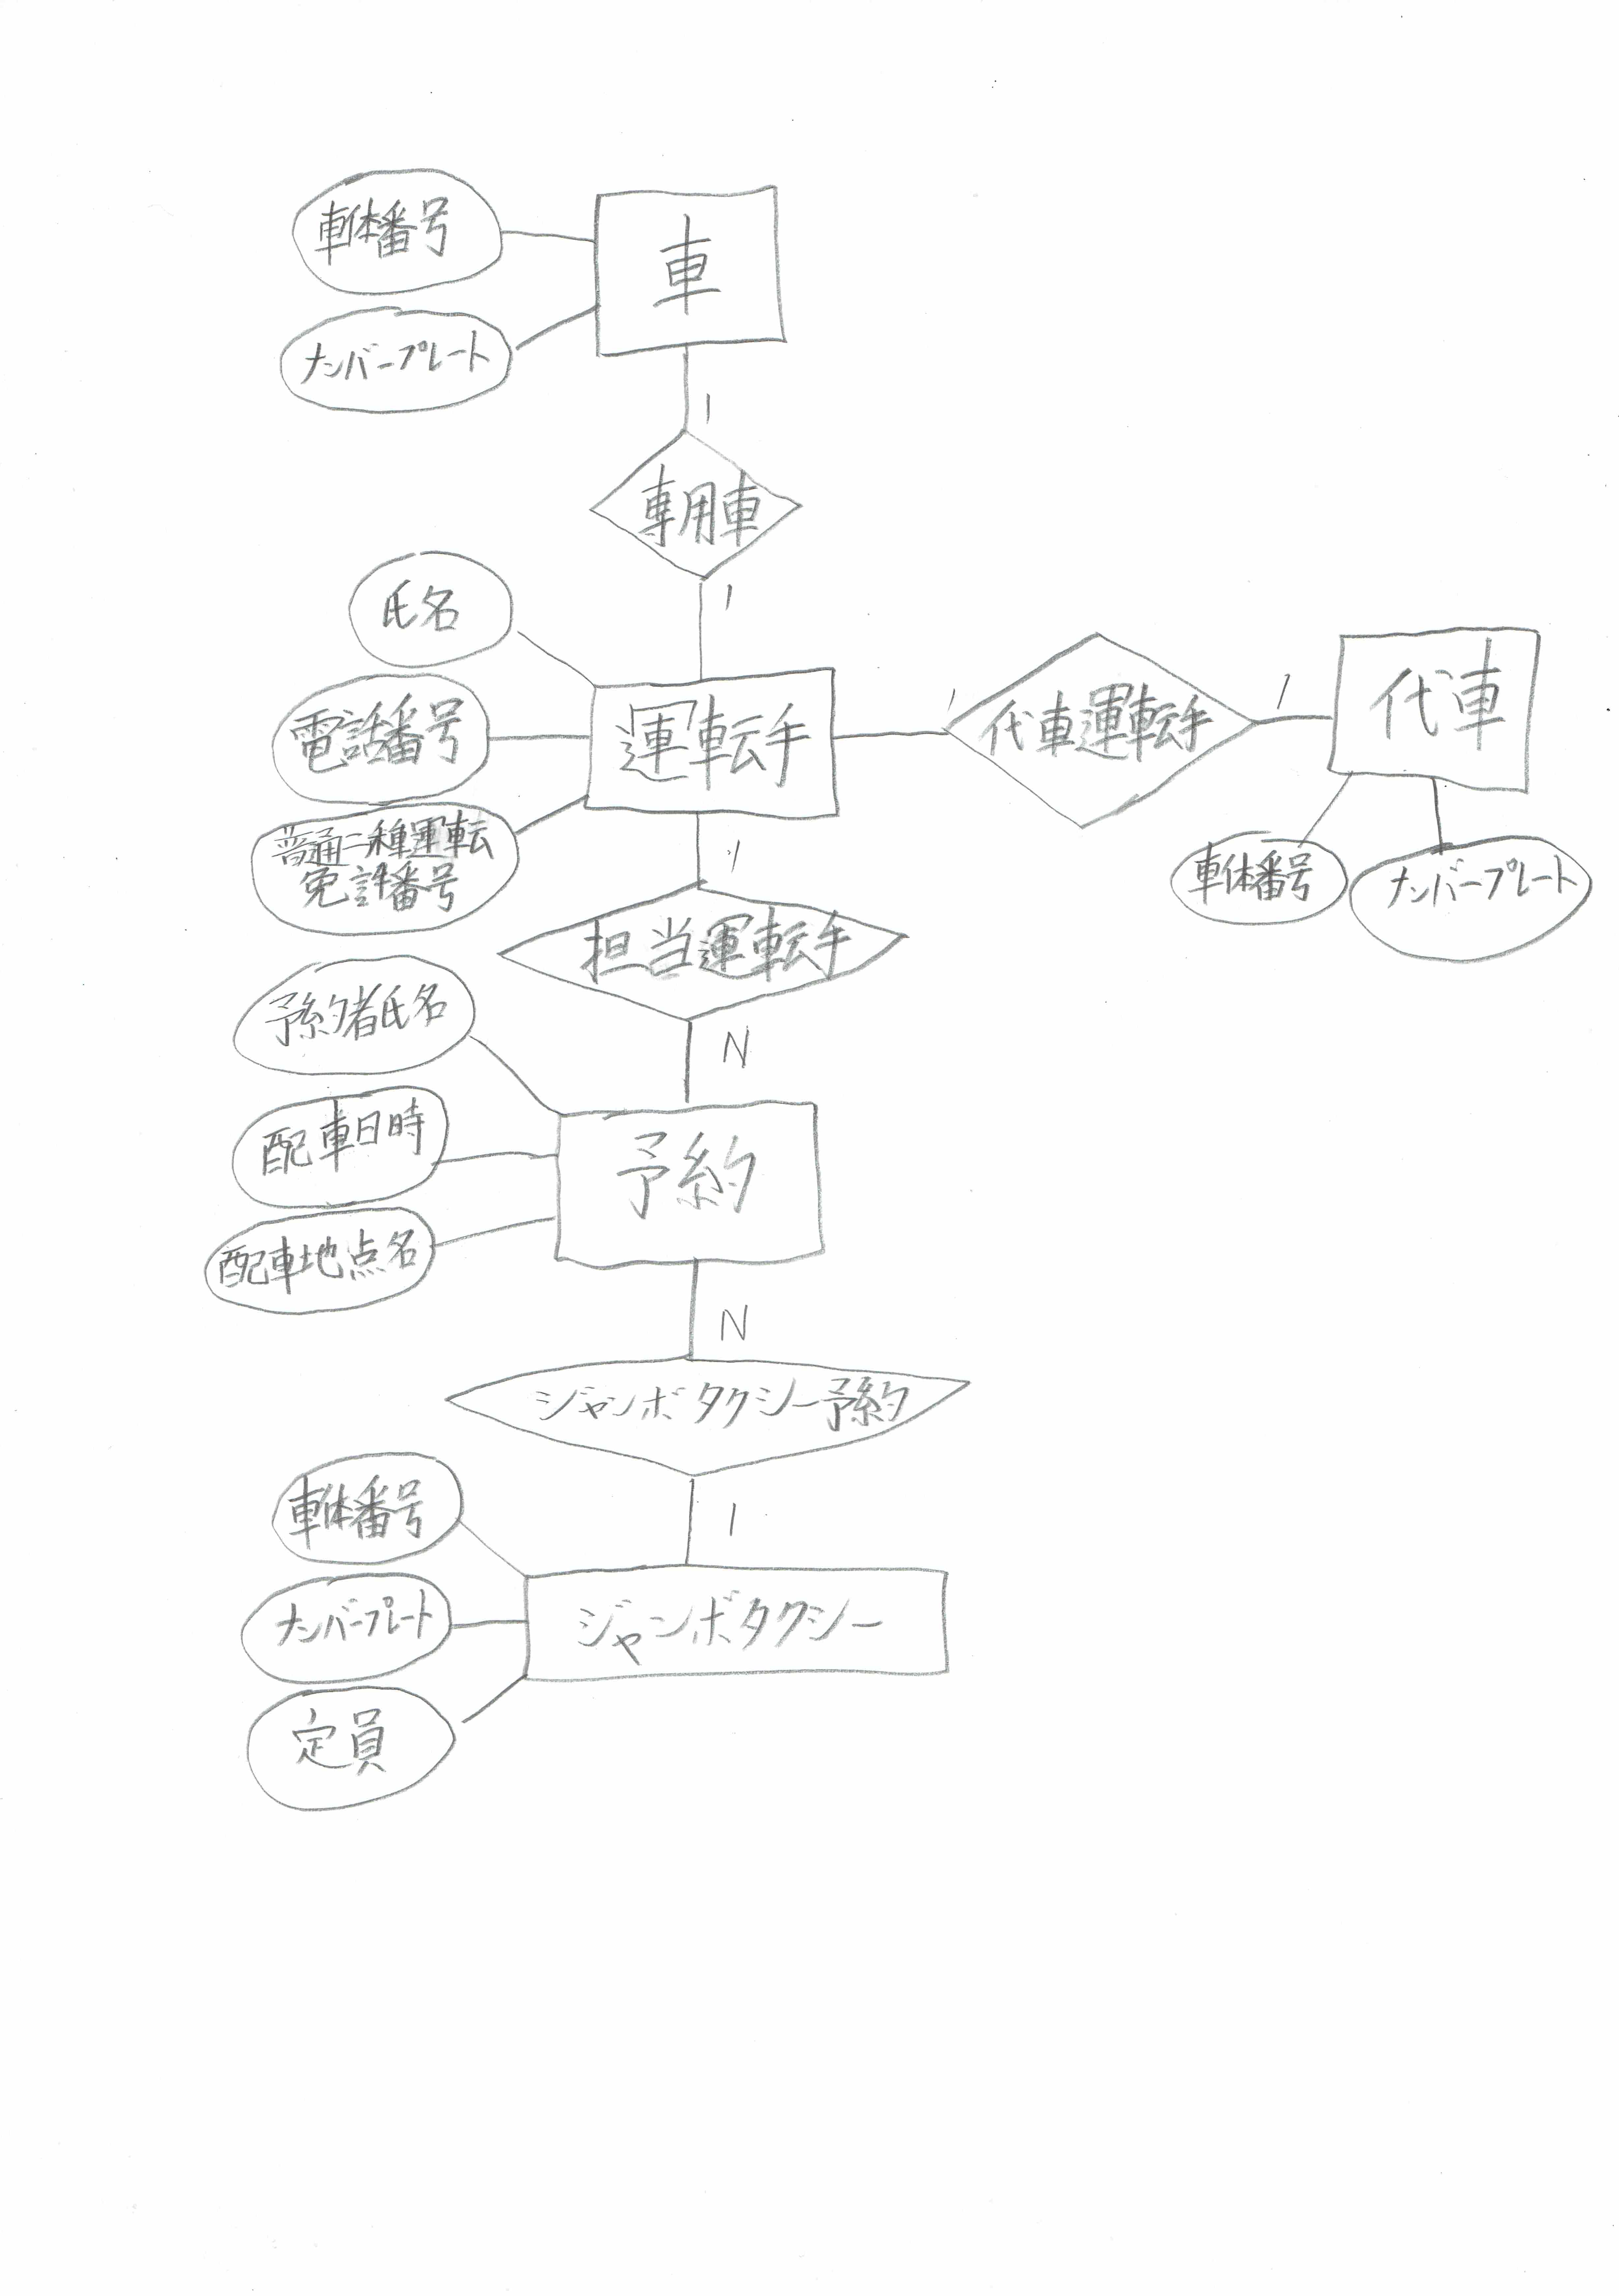
\includegraphics[width=15cm]{PeterChen.JPG}
\end{document}
